\chapter{Resultados}
\section{Geração do conjunto de imagens de teste}
As imagens usadas para testar o método de restauração descrito neste trabalho foram geradas artificialmente a partir de uma única imagem usando o modelo de observação descrito na seção \ref{sec:obsmodel}.
Para os testes reportados aqui foi usada a imagem da Figura \ref{fig:hrimage}.
Usando o modelo de observação, foram geradas 20 imagens de baixa resolução como as da Figura \ref{fig:frames}.
Para diminuir o custo computacional do processo, a imagem foi convertida para escala de cinza antes da degradação.

\begin{figure}[h]
	\centering
	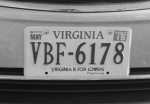
\includegraphics{figures/imtestes.png}
	\caption{Imagem de alta resolução utilizada nos testes.}
	\label{fig:hrimage}

\end{figure}

Para os testes feitos neste trabalho, a imagem de alta resolução foi reamostrada de forma que as dimensões das imagens de baixa resolução são iguais a $0.25$ vezes as dimensões da imagem HR.  
Dessa forma, há 16 pontos na image de alta resolução para cada ponto na imagem de baix resolução.
A largura da função de espalhamento de ponto ($\gamma$) escolhida foi 2.
Para cada imagem, o ângulo de rotação foi escolhido aleatoriamente de uma distribuição uniforme entre $-4$ e $4$ graus.
A mesma seleção aleatória foi feita para o deslocamento linear da imagem; a quantidade de pontos de deslocamento foi retirada de uma distribuição uniforme e contínua entre $-2$ e $2$ em cada um dos eixos.
A tabela \ref{tab:resumoParametros} resume os parâmetros utilizados na degradação das imagens.

\begin{figure}[H]
	\centering
	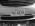
\includegraphics{figures/degradedImg/result-0.png}
	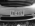
\includegraphics{figures/degradedImg/result-1.png}
	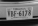
\includegraphics{figures/degradedImg/result-2.png}
	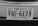
\includegraphics{figures/degradedImg/result-3.png}
	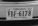
\includegraphics{figures/degradedImg/result-4.png}
	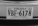
\includegraphics{figures/degradedImg/result-5.png}
	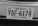
\includegraphics{figures/degradedImg/result-6.png}
	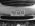
\includegraphics{figures/degradedImg/result-7.png}
	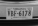
\includegraphics{figures/degradedImg/result-8.png}
	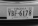
\includegraphics{figures/degradedImg/result-9.png} \\
	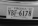
\includegraphics{figures/degradedImg/result-10.png}
	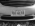
\includegraphics{figures/degradedImg/result-11.png}
	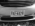
\includegraphics{figures/degradedImg/result-12.png}
	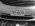
\includegraphics{figures/degradedImg/result-13.png}
	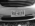
\includegraphics{figures/degradedImg/result-14.png}
	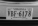
\includegraphics{figures/degradedImg/result-15.png}
	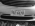
\includegraphics{figures/degradedImg/result-16.png}
	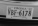
\includegraphics{figures/degradedImg/result-17.png}
	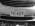
\includegraphics{figures/degradedImg/result-18.png}
	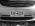
\includegraphics{figures/degradedImg/result-19.png}
	\caption{Conjunto das imagens geradas a partir da imagem de alta resolução. Note a diferença sutil entre as imagens causada pelas transformações de deslocamento e rotação.}
	\label{fig:frames}
\end{figure}

\begin{table}[h]
	\centering
	\caption{Parâmetros de degradação usados para gerar o conjunto de imagens de teste.}
	\label{tab:resumoParametros}
	\begin{tabular}{r | l}
		Ângulos de rotação ($\theta_k$) & $ \sim \mathcal{U}(-4, 4)$ \\ \hline
		Deslocamento ($\mathbf{s}_k$)& $\sim \mathcal{U}(-2,2)$\\ \hline
		Largura da PSF ($\gamma$) & 2 \\ \hline
		Dimensões da imagem de alta resolução & XXXX \\ \hline
		Dimensões das imagens de baixa resolução & CCC \\

	\end{tabular}

\end{table}
